\chapter{Line Fitting}

\begin{introduction}[Keywords]
    \item 最小二乘法 Least Square Method
    \item 奇异值分解 Singular Value Decomposition (SVD)
    \item 随机抽样一致算法 RANdom SAmple Consensus (RANSAC)
    \item 霍夫变换 Hough Transform
    \item 鲁棒性 Robustness
    \item 离群点 Outliers
    \item 内点 Inliers
\end{introduction}

\section{Least Square Method}

最小二乘法想必都熟知

\begin{figure}[htbp]
    \centering
    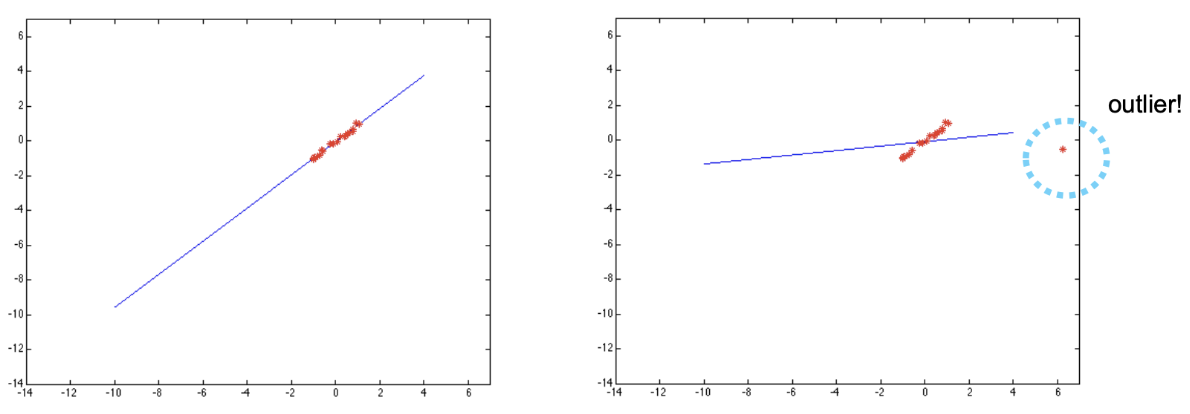
\includegraphics[width=0.8\textwidth]{figures/not_roboust_outliner.png}
    \caption{Least Square Method is not robust to outliers}
\end{figure}

对细微噪声\textbf{鲁棒(robust)}, 但是对于\textbf{离群点(Ouliers)}敏感.

\href{http://faculty.bicmr.pku.edu.cn/~wenzw/bigdata/matrix-cook-book.pdf}{Matrix Cookbook} : 记录了很多矩阵求导的公式

\section{Singular Value Decomposition (SVD)}

SVD 这里的作用在于, 对给定一组数据点, 找到最适配的 k 维子空间, 使得所有数据点到这个子空间的距离最小. 这里我认为王鹤老师讲解地不够本质, 但 SVD 本身非常基础, 可以自行查阅资料.

\newpage
\section{RANSAC}


RANSAC : RANdom SAmple Consensus

Idea: we need to find a line that has the largest supporters (or inliers)

\begin{definition}[RANSAC loop]
    假设这个直线 (平面) 需要两个 (n个) 点来确定 : 

    \begin{enumerate}
        \item 随机选择 k 组能确定这个直线的点,也就是在所有点里面选出一个 $k\times 2$ 的矩阵
        \item 对每一组点计算出一条直线 (SVD)
        \item 对每一组点的直线计算出所有点到这条直线的距离,如果小于阈值,则认为这个点是这条直线的 inlier
        \item 找到最大的 inlier 数量的直线,如果大于阈值,则认为这条直线是最优的
        \item 对这个最优的直线,用这个直线所有的 inlier 重新计算一次直线
        \item 重复上述步骤, 直到 inlier 数量不再增加
    \end{enumerate}
    
\end{definition}
\begin{note}
    实际上从今天来看这个 loop 不需要, 因为我们可以并行地提出所有假设 (Hypothesis), 这里王鹤老师留作作业.
\end{note}

\section{RANSAC calculation}
\begin{problem}
假设我们有所有 inliner 占比为 $w$ 的先验知识,同时希望有不低于 $p$ 的概率能够找到一个最优的直线,那么我们需要多少次迭代呢?
\end{problem}
\begin{proof}
注意到, 
\begin{equation}
\mathbf{\Pr}\text{[一组点全部是inliner]} = w^n
\end{equation}

如果一组点中有一个点是 outliner,那么我们称这组点 fail.

\begin{equation}
\mathbf{\Pr}\text{[k组点全部fail]} = {(1-w^n)}^k
\end{equation}

我们希望 k 组点全部 fail 的概率小于 $1-p$.

\begin{equation}
{(1-w^{n})}^k < 1-p
\Rightarrow
k > \frac{\log(1-p)}{\log(1-w^n)}
\end{equation}
\end{proof}

\newpage
\section{Hough Transform}

其实就是把一条直线从实际空间的表示转换到参数空间的表示. 但是如果存在垂直的直线, 可能需要考虑使用极坐标来作为参数空间.

\begin{figure}[htbp]
    \centering
    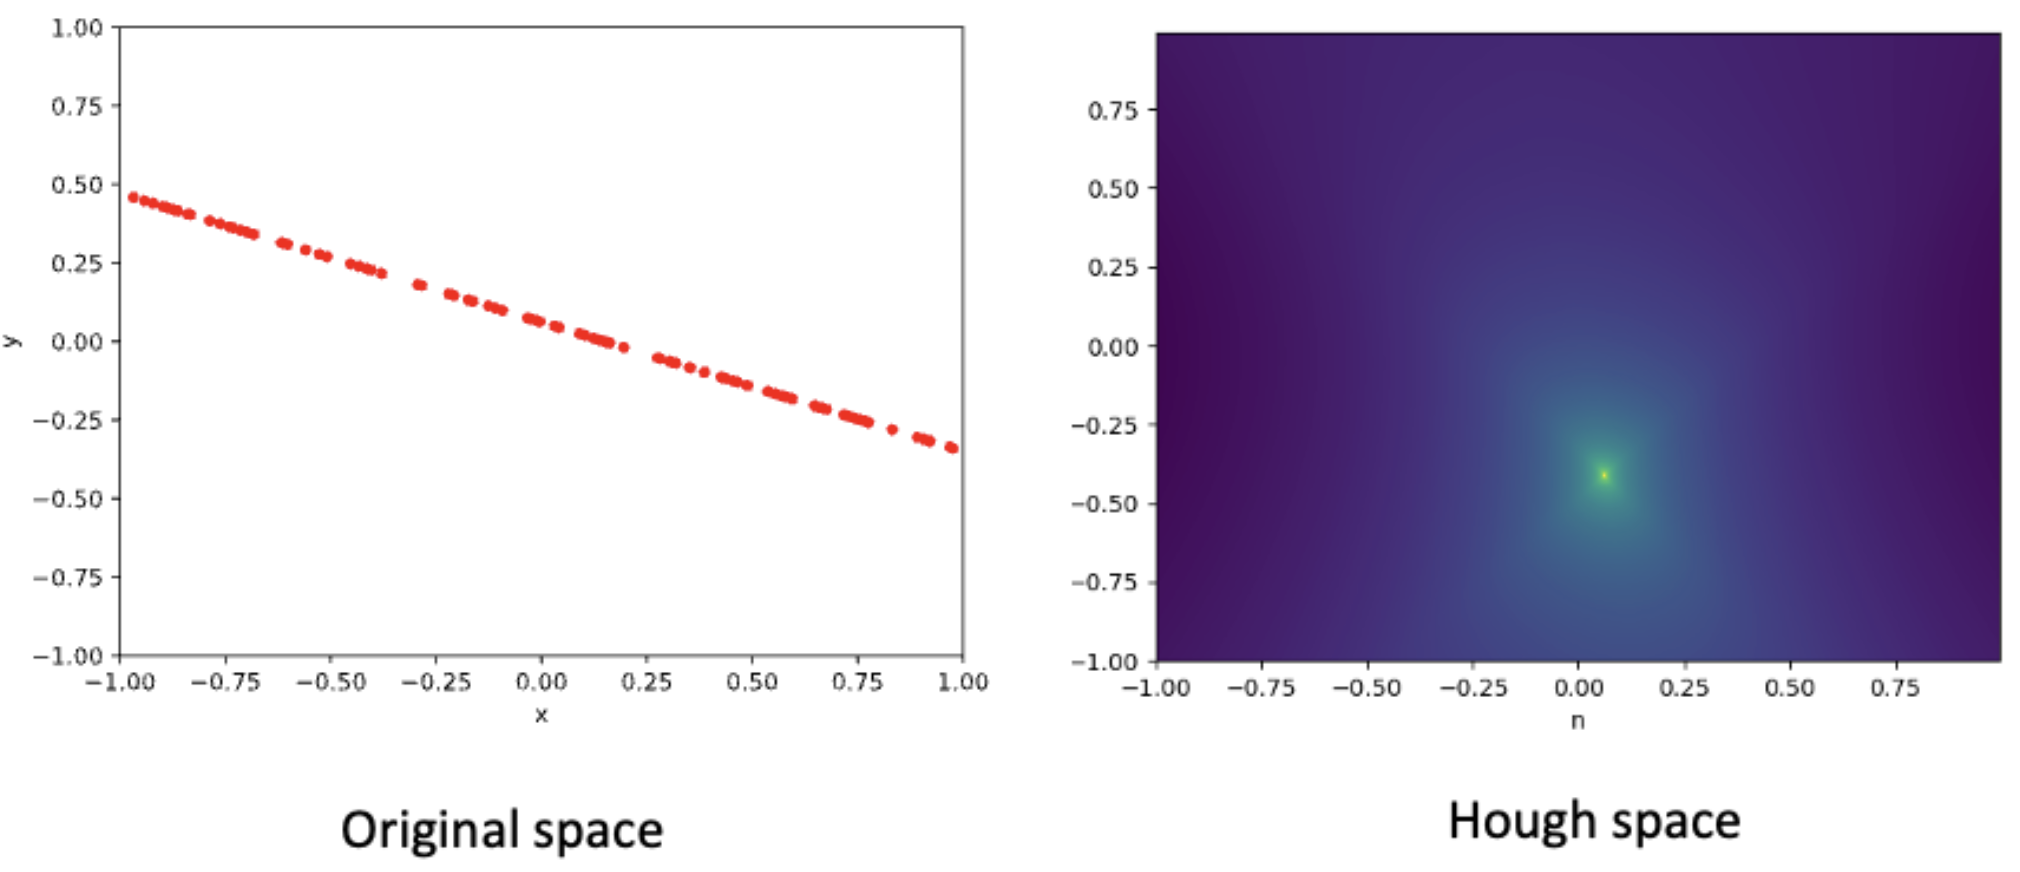
\includegraphics[width=0.8\textwidth]{figures/hough1.png}
    \caption{Hough Transform w/o Noise}
\end{figure}

\begin{figure}[htbp]
    \centering
    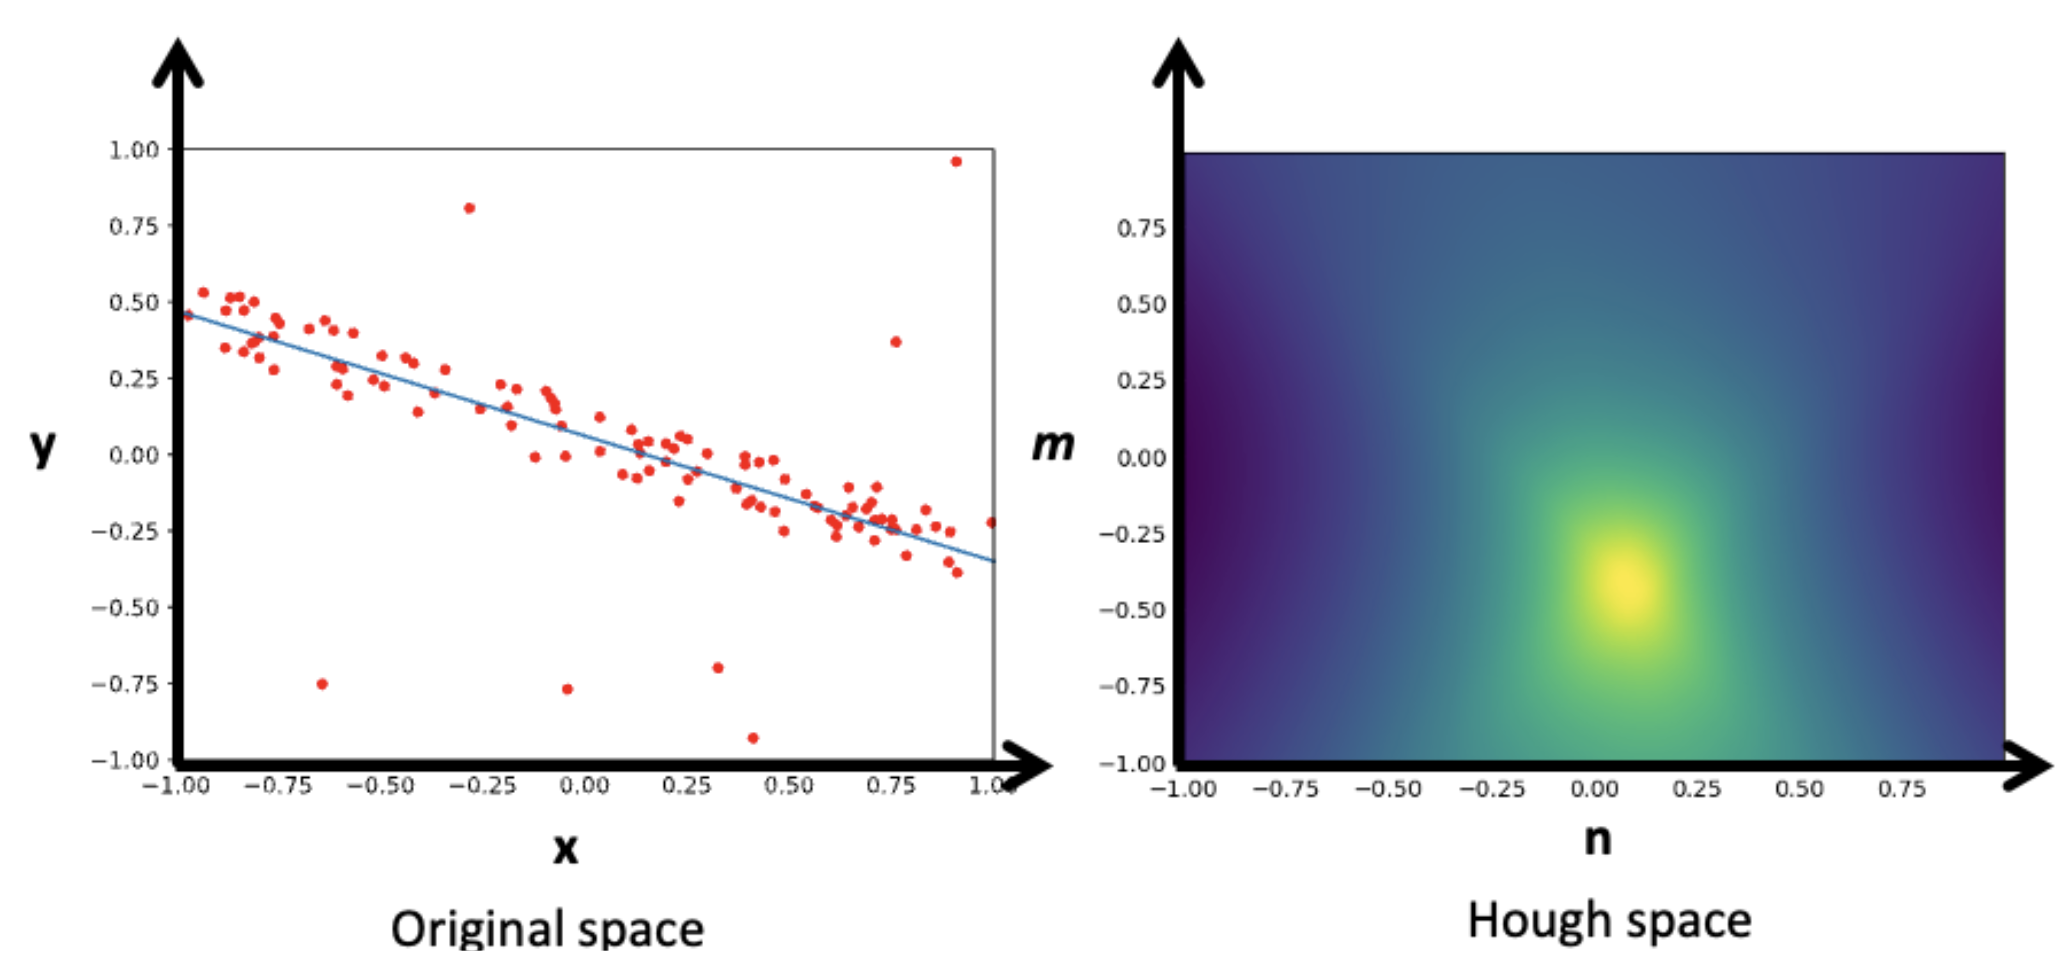
\includegraphics[width=0.8\textwidth]{figures/hough2.png}
    \caption{Hough Transform w/ Noise and Outliers}
\end{figure}